% !TEX root = ../main.tex
\chapter{Gestión del Proyecto}

\section{Metodología elegida}
Para el desarrollo del proyecto se adoptó una metodología ágil evolutiva, en la cual el sistema se construyó y refinó a través de ciclos sucesivos de desarrollo. Cada iteración produjo un incremento funcional del producto, permitiendo validar decisiones de diseño y ajustar requisitos a medida que el proyecto avanzaba. Esta metodología resultó especialmente adecuada para el presente proyecto, dado que la incorporación progresiva de integraciones con APIs externas y la naturaleza exploratoria de algunas funcionalidades requieren de flexibilidad para incorporar cambios sin comprometer la estructura general del desarrollo.

El equipo, compuesto por tres integrantes, organizó el trabajo en iteraciones de dos semanas. Al inicio de cada iteración se definían las tareas a abordar a partir del backlog priorizado, y al cierre se evaluaba el avance y se ajustaba la planificación para la siguiente. No se adoptaron roles fijos, siendo el equipo responsable colectivamente de la planificación, el desarrollo y la validación de cada incremento.

\section{Herramientas de gestión}
\begin{table}[H]
  \centering
  \renewcommand{\arraystretch}{1.25}
  \begin{tabularx}{\textwidth}{>{\bfseries}l X}
    \toprule
    Herramienta & Uso \\
    \midrule
    Jira & Backlog, issues y seguimiento de iteraciones \\
    Bitbucket & Espejo del repositorio de GitHub, integrado con Jira \\
    GitHub & Repositorio principal, control de versiones y gestión de PRs \\
    GitHub Actions & Integración continua: ejecución de los tests y replicación del repositorio en Bitbucket \\
    \bottomrule
  \end{tabularx}
  \caption{Herramientas de gestión}
  \label{tab:herramientas_gestion}
\end{table}

La integración nativa entre Jira y Bitbucket permitió referenciar commits y PRs directamente desde cada issue, brindando trazabilidad completa entre las tareas planificadas y el código desarrollado. Esta combinación de herramientas coincide además con uno de los casos de uso centrales del sistema desarrollado, lo que le permitió al equipo validar en primera persona las integraciones que el producto busca ofrecer.

\section{Fases del proyecto}
\begin{table}[H]
  \centering
  \renewcommand{\arraystretch}{1.25}
  \begin{tabularx}{\textwidth}{>{\bfseries}p{0.34\textwidth} X}
    \toprule
    Fase & Descripción \\
    \midrule
    Interfaz gráfica y persistencia de los nodos. & Esta fase abarcó el MVP, que consistió en producir una interfaz visual usable donde los cambios del grafo persisten para mantener el estado entre usos. Sentó las bases para el resto del proyecto. \\
    Integración con APIs preestablecidas & En esta fase se desarrolló el módulo principal del proyecto, la información en tiempo real. Se logró la integración con diversas APIs para dar opciones a los usuarios no técnicos a obtener información actualizada de temas de interés general, como vuelos y estadías. \\
    Integración personalizada con APIs de terceros & Se extendió lo logrado en la fase anterior, permitiendo integración con APIs de forma personalizada. \\
    Monetización & Se planificó implementar el sistema de pagos para los distintos tiers según el uso de la aplicación (por ejemplo, límite de conexiones, refresh rates fijos, o número de tableros por usuario). El análisis económico de los planes se presenta en el Capítulo~\ref{chap:monetizacion}. \\
    Investigación sobre memoria de agentes & Se estudió el manejo de memorias de agentes de IA, aprovechando la interfaz del sistema para representar las entradas guardadas en forma de grafo, y darle a los usuarios la flexibilidad de customizar o corregir los nodos de la memoria. \\
    Implementación del caso de uso de memorias de agentes (condicional) & Ante los resultados positivos de la investigación, se desarrolló el módulo de la aplicación que permite adaptar el caso de uso. \\
    Desarrollo de API y/o MCP para accesos internos a la herramienta & Ya con un sistema robusto desarrollado y funcionando, se buscó brindar mediante una API/MCP server exponer una nueva forma de acceder a la información almacenada ya no solo mediante la interfaz gráfica sino también desde aplicaciones de terceros e incluso accesible para agentes mediante un servidor MCP. \\
    \bottomrule
  \end{tabularx}
  \caption{Fases del Proyecto}
  \label{tab:fases_proyecto}
\end{table}

\section{Cronograma}
En base a la complejidad de las tareas, en conjunto a la disponibilidad del equipo y los períodos de los sprints, se desarrolló el siguiente diagrama de Gantt con el camino crítico del desarrollo del proyecto:

\begin{figure}[H]
  \centering
  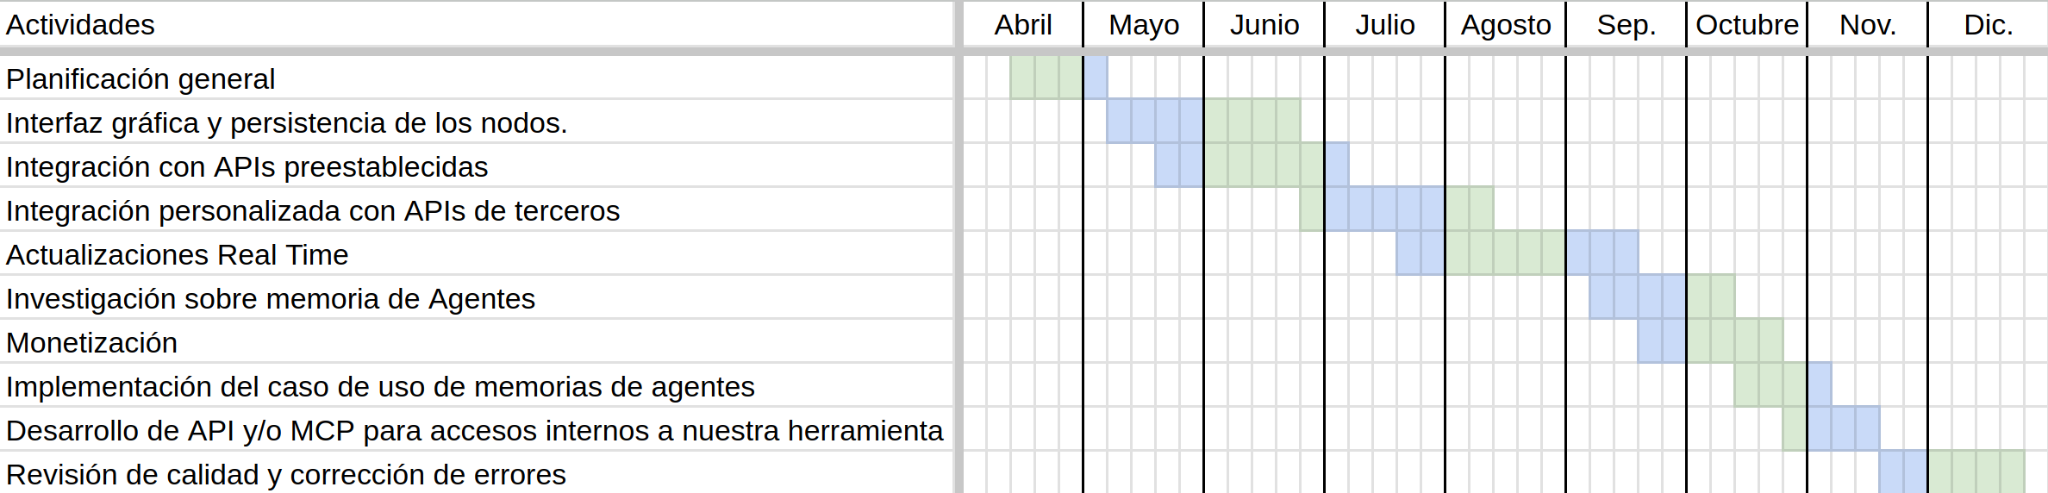
\includegraphics[width=\textwidth]{figuras/fig01.png}
  \caption{Cronograma del proyecto}
  \label{fig:cronograma_inicial}
\end{figure}

\section{Ejecución real del proyecto}
El trabajo se desarrolló de forma ordenada y estructurada, siguiendo el diagrama de Gantt presentado en la sección anterior. Sin embargo, se produjo un desvío con la organización original, dado que se decidió postergar la implementación del sistema de monetización hasta luego de integrar el servicio de MCPs en el producto.

La Figura~\ref{fig:cronograma_actualizado} presenta el cronograma actualizado, en el cual la fase de monetización se desplaza al final del proyecto, luego del desarrollo de la API y del servidor MCP, y se incorporan las actualizaciones en tiempo real y una etapa final de revisión de calidad y corrección de errores.

\begin{figure}[H]
  \centering
  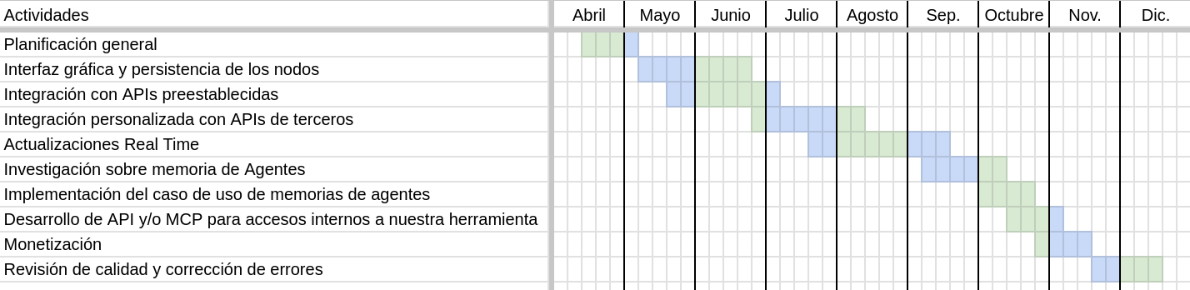
\includegraphics[width=\textwidth]{figuras/fig02.png}
  \caption{Cronograma del proyecto actualizado}
  \label{fig:cronograma_actualizado}
\end{figure}

Las tareas se distribuyeron entre los integrantes del equipo de forma equitativa, estableciendo objetivos bimensuales y reuniones semanales de avances. Esta organización le dio al equipo gran flexibilidad de desarrollo y autogestión, permitiendo a cada uno enfocarse en la tarea a mano.

\section{Gestión de riesgos}
Durante la planificación se identificaron los principales riesgos que podían afectar el desarrollo y el funcionamiento del sistema. La Tabla~\ref{tab:riesgos} resume cada uno de ellos junto con el tratamiento adoptado, que en la mayoría de los casos se incorporó al propio diseño de la solución.

\begin{table}[H]
  \centering
  \renewcommand{\arraystretch}{1.25}
  \begin{tabularx}{\textwidth}{>{\bfseries}p{0.35\textwidth} X}
    \toprule
    Riesgo & Tratamiento \\
    \midrule
    Cambios o caída de las APIs de terceros & Cada tarjeta muestra su error sin afectar al resto del tablero, y las integraciones del catálogo pueden corregirse desde la aplicación sin desplegar una nueva versión. \\
    Límites de uso de las APIs externas & El resultado de cada tarjeta se guarda en caché durante el tiempo configurado, de modo que cada API se consulta como máximo una vez por período. \\
    Filtración de credenciales de los usuarios & Los valores se cifran con AES-GCM por ámbito, nunca se devuelven por la API y las peticiones salientes se realizan con un cliente HTTP que bloquea direcciones internas. \\
    Límites de los planes gratuitos de Vercel, MongoDB Atlas y Redis Cloud & El sistema puede desplegarse también con Docker, y la migración a AWS se planifica al superar los 500.000 usuarios y se ejecuta antes de alcanzar 1.000.000 (Capítulo~\ref{chap:monetizacion}). \\
    Disponibilidad del equipo & El trabajo se organizó en iteraciones de dos semanas, con una replanificación al cierre de cada una. \\
    Cambios en el protocolo MCP, de reciente aparición & El servidor MCP se mantiene separado del backend y consume su API REST, por lo que puede actualizarse de forma independiente. \\
    \bottomrule
  \end{tabularx}
  \caption{Riesgos del proyecto y su tratamiento}
  \label{tab:riesgos}
\end{table}